\documentclass[11pt,answers]{exam}

\usepackage{etex}
\usepackage{amssymb,amsmath,multicol} %<-- InWorksheetExam1 i also have fancyhdr,

\usepackage[metapost]{mfpic}
\usepackage[pdftex]{graphicx}

\usepackage{pst-plot}
\usepackage{pgfplots}
\pgfplotsset{compat=1.9}

\usepackage{tikz}
\usepackage{tkz-2d}
\usepackage{tkz-base}
\usetikzlibrary{calc}
\usepackage{tabu}

\usepackage[inline]{enumitem}
\usepackage{refcount}%<-- non in WorksheetExam1

\usepackage{caption}

\usepackage{array}
\newcolumntype{L}[1]{>{\raggedright\let\newline\\\arraybackslash\hspace{0pt}}m{#1}}
\newcolumntype{C}[1]{>{\centering\let\newline\\\arraybackslash\hspace{0pt}}m{#1}}
\newcolumntype{R}[1]{>{\raggedleft\let\newline\\\arraybackslash\hspace{0pt}}m{#1}}

%\renewcommand{\headrulewidth}{0pt}

\newcommand{\vasymptote}[2][]{
    \draw [densely dashed,#1] ({rel axis cs:0,0} -| {axis cs:#2,0}) -- ({rel axis cs:0,1} -| {axis cs:#2,0});
}

\addpoints
%\printanswers
\noprintanswers

\opengraphsfile{Exam1A_Spring_2016}

\begin{document}
\extrawidth{-0.3in}
\pagestyle{headandfoot}

\setlength{\hoffset}{-.25in}

\extraheadheight{-.4in}
\runningheadrule
\firstpageheader{\bfseries {MATH1-UC 1171}}{ \bfseries {Exam 1 }}{\bfseries {3/8/2016}} 



\firstpagefooter{\bfseries{}}{}{} 


\runningheader{\bfseries {}}%
              {\bfseries {}}%
              {Page \thepage\ 
							of \numpages 
							}
\runningfooter{} %%&&CHANGED
                {}
                {Points earned: \hbox to 0.5in{\hrulefill}
                 out of  \pointsonpage{\thepage} points}
                 
						

\vspace*{0.7cm}
\hbox to \textwidth { \scshape {Name:} \enspace\hrulefill}
\vspace{0.2in}

\begin{itemize}
	\item This exam contains \numpages\ pages, including this cover page and the blank last page which you can tear out and use as scrap paper. Enter
your name on the top of this page, and put your initials
on the top of every page. Please note that I will not grade anything that you write on the last (blank) page.

%\item Please read the instructions for each individual problem carefully. Try not to overthink a problem and read between the lines! Take your time to solve each problem, and don't rush to finish!
%\item Write legibly and clearly label your answers. If I cannot read your solution to a problem, the problem will receive a score of zero.
\item Calculators may not be used in this exam. You may use your note-card with fomulas/examples. 

\item Please write your name on your note-card and include it in your exam. If you do not have a note-card, please write {\textit {no note-card}} on this page.
\item Turn off all phones and computers, and remove all headphones.

\end{itemize}

For the problems where you are required to show your work, the following rules apply:\\

\begin{minipage}[t]{3.7in}
\vspace{0pt}
\begin{itemize}

\item \textbf{Write in complete sentences}, explaining your calculations, graphs and tables. If you draw a graph, you must label the axes, include tick marks and include units both on the horizontal and vertical axis. If you are asked to explain in practical terms, then your explanation cannot contain math symbols or formulas.
\item \textbf{Use the methods described in this course} as part of your explanations: for example, you cannot use derivatives to find the peaks and valley of a function.

\item \textbf{Organize your work}, neatly and legibly in
the space provided. Work that is disorganized and difficult to read will not receive full credit.  

\item \textbf{A correct answer, unsupported by calculations, explanation,
or algebraic work will receive no credit}; an incorrect answer supported
by  calculations and explanations may receive
partial credit.


\item \textbf{If you need more space}, use the back of the pages; clearly indicate when you have done this.
\end{itemize}

Do not write in the table to the right.
\end{minipage}
\hfill
\begin{minipage}[t]{2.3in}
\vspace{0pt}
%\cellwidth{3em}
\gradetablestretch{2}
\vqword{Pages}
\addpoints % required here by exam.cls, even though questions haven't started yet.	
\combinedgradetable[v][pages]  % Use [pages] to have grading table by page instead of question

\end{minipage}
\newpage

%\bigskip

%\begin{center}
%\gradetable[v][pages]
%\end{center}

%\newpage

\pointpoints{point}{points}

\begin{questions}


\addpoints

\question[2] Find the $x$ and $y$ intercepts of the rational function $\displaystyle r(x) = 
\frac{2}{x^2 + 5x - 3}$. (If an answer does not exist, enter DNE.)


{\tabulinesep=1.2mm
	\begin{tabu}{c  c c c c c c }
		
		$x$ intercept   & $(x,y)=$ & $(\hbox to 0.5in{\hrulefill},\hbox to 0.5in{\hrulefill})$    & &	
		$y$ intercept   & $(x,y)=$ & $(\hbox to 0.5in{\hrulefill},\hbox to 0.5in{\hrulefill})$    \\ 
	\end{tabu}}
	\vskip 0.2cm

\question[1] The graph of the function $\displaystyle f(x)=\frac{x(x+1)}{(x-2)^4}$ intersects the horizontal asymptote of the function.
\begin{oneparchoices}
	\choice True \choice False
	\end{oneparchoices} 
	
	\question[1] The graph of the function $\displaystyle f(x)=\frac{1}{x}$ intersects the horizontal asymptote of the function.
	\begin{oneparchoices}
		\choice True \choice False
	\end{oneparchoices} 
\question Let $\displaystyle r(x)=\frac{3x^2-7x+2}{4x^2+11x+13}$.
\begin{parts}
	\part[1] As $x\to \infty$, $r(x)\to \hbox to 0.8in{\hrulefill}$
	\part[1] As $x\to -\infty$, $r(x)\to \hbox to 0.8in{\hrulefill}$
	\end{parts}

\question[1] There is a function for which the two statements below are true simultaneously:
\begin{itemize}
	\item The graph of the function passes the horizontal line test, and
	\item The graph of the function fails the vertical line test.
\end{itemize}

\begin{oneparchoices}
	\choice True \choice False
\end{oneparchoices} 

\question The complete graph of a function $f(x)$ is given below.

\begin{center}
	
	\begin{mfpic}[20]{-1}{6}{-2}{5}
		
		%\polyline{(0,-2), (4,1), (4,2), (5,3)}
		
		\polyline{(0,2), (5,1)} 
		
		%\polyline{(4,2), (5,2)}
		
		\point[5pt]{(0,2),  (5,2)}
		\circle{(5, 1),0.15}
		

		
		\axes
		
		\xmarks{1,2,3,4,5}
		
		\ymarks{-2,-1,1,2,3,4,}
		
		\tlpointsep{4pt}
		
		\axislabels {x}{{\tiny $1$} 1, {\tiny $2$} 2, {\tiny $3$} 3, {\tiny $4$} 4, {\tiny $5$} 5}
		
		\axislabels {y}{{\tiny $1$} 1,{\tiny $2$} 2, {\tiny $3$} 3, {\tiny $4$} 4,  {\tiny $-1$} -1, {\tiny $-2$} -2}
		
		% Grid
		%\drawcolor[gray]{0.25}
		%\gridlines{1, 1}
		\drawcolor[gray]{0.75} 
		\grid{1,1}
		
	\end{mfpic}
	
\end{center}

\begin{parts}
	\part[1] $f(0)=$\dotfill
	\part[1] The domain (in interval form) is \dotfill
	\part[1] The range (in interval form) is \dotfill
	\part[4] Write a formula for $f(x)$.
	\fillwithdottedlines{1cm}
	
\end{parts}
\question[2] Do the tails of the rational function $\displaystyle r(x)=\frac{(x-1)(x-2)}{(x-6)^3}$ near its vertical asymptote go in the same direction or in opposite direction? How do you know?
\fillwithdottedlines{2cm}

\newpage
\question[1]  A school fund-raising group sells chocolate bars to help finance a swimming pool for their physical education program. 
The group finds that when they set their price at $x$ dollars per bar (where 
$0 < x \leq 5$), their total sales revenue (in dollars) is given by the function 
$\displaystyle R(x) = −500x^2 + 3000x$. What do these values represent? (Circle the best answer.)

\begin{choices}
	\choice $R(2)$ and $R(4)$ represent their total expenses when their price is \$2 and \$4 per bar respectively.
	
	\choice $R(2)$ and $R(4)$ represent their total profits when their price is \$2 and \$4 per bar respectively.
	
	
	\choice $R(2)$ and $R(4)$ represent their total sales revenue when their price is \$2 and \$4 per bar respectively.
	
	\choice $R(2)$ and $R(4)$ represent their total profits when their profit is \$2 and \$4 per bar respectively.
	
	\choice $R(2)$ and $R(4)$ represent their total expenses when their expense is \$2 and \$4 per bar respectively.
\end{choices}

\question The graph of a function $f(x)$ is shown below.



\begin{center}
	
	\begin{mfpic}[20]{-1}{6}{-2}{5}
		
		%\polyline{(0,-2), (4,1), (4,2), (5,3)}
		
		\polyline{(0,1), (1,4)} 
		
		\polyline{(1,4), (2,2)}
		
		\polyline{(2,2), (3,4)}
		
		\polyline{(3,4), (4,1)}
		
		\point[5pt]{(0,1), (4,1)}

		
		\tcaption{\scriptsize $y=f(x)$}
		
		\axes
		
		\xmarks{1,2,3,4,5}
		
		\ymarks{-2,-1,1,2,3,4,}
		
		\tlpointsep{4pt}
		
		\axislabels {x}{{\tiny $1$} 1, {\tiny $2$} 2, {\tiny $3$} 3, {\tiny $4$} 4, {\tiny $5$} 5}
		
		\axislabels {y}{{\tiny $1$} 1,{\tiny $2$} 2, {\tiny $3$} 3, {\tiny $4$} 4,  {\tiny $-1$} -1, {\tiny $-2$} -2}
		
		% Grid
		%\drawcolor[gray]{0.25}
		%\gridlines{1, 1}
		\drawcolor[gray]{0.75} 
		\grid{1,1}
		
	\end{mfpic}
	
\end{center}

\begin{parts}
	\part[3] Fill out the table shown below. (Your answers should be exact values, not estimates. If an answer does not exist, enter DNE.)
	\vskip 0.5cm
		
	\begin{minipage}{\linewidth}
		\centering
		%\captionof{table}{} \label{tab:ettobbotte}  
		\begin{tabular}{L{1.5cm}|C{0.8cm}|C{0.8cm}|C{0.8cm}|C{0.8cm}|C{0.8cm}|C{0.8cm}|C{0.8cm}}
			%\hline
			$x$    & $-1$ & $0$ &  $1$ &  $2$ & $3$ & $4$ & $5$ \\ \hline
			$f(x+1)$ &      &     &     &     &     &       & \\ 
		\end{tabular}
	\end{minipage}
	\vskip 0.5cm
		
	\part[3] Fill out the table shown below. (Your answers should be exact values, not estimates. If an answer does not exist, enter DNE.)
	\vskip 0.5cm
		
	\begin{minipage}{\linewidth}
		\centering
		%\captionof{table}{} \label{tab:ettobbotte}  
		\begin{tabular}{L{1.5cm}|C{0.8cm}|C{0.8cm}|C{0.8cm}|C{0.8cm}|C{0.8cm}|C{0.8cm}|C{0.8cm}}
			%\hline
			$x$    & $-1$ & $0$ &  $1$ &  $2$ & $3$ & $4$ & $5$ \\ \hline
			$-2f(x)$ &      &     &     &     &     &       & \\ 
		\end{tabular}
	\end{minipage}
		\vskip 0.5cm
	\part[1] The range of $f(-x)$ is $[0,4]	$. 
	\begin{oneparchoices}
		\choice True \choice False
		\end{oneparchoices}
		\bonuspart[2] Write a formula for $f(x)$. (Hint: The formula has four parts.)
		\fillwithdottedlines{2cm}
	\end{parts}

%\newpage


\question \label{question:queoca} A polynomial function $P(x)$  has all of the following properties.
\begin{itemize}
	\item As $x\to -\infty$, $P(x)\to \infty$;
	\item As $x\to \infty$, $P(x)\to -\infty$;
	\item $(0,0)$ is one of the two $x$ intercepts, and the graph of $P(x)$ bounces off the $x$ axis at $x=0$;
	\item $(4,0)$ is the other $x$ intercept, and the graph of $P(x)$ goes across the $x$ axis at $x=4$.
\end{itemize}
\begin{parts}
	\part[2] Is the degree of $P(x)$ even or odd? How do you know?
	\fillwithdottedlines{1.5cm}
	\part[1] Write the domain of $P(x)$ in interval form. \dotfill
	\part[2] \label{part:partettob} On the grid provided below, draw a possible graph for $P(x)$.
	
	
	
\begin{tikzpicture}
	\draw[gray!50, thin, step=0.5] (-7,-3) grid (7,3);
	\end{tikzpicture}

\part[2] Does the graph in part~(\ref{part:partettob}) show a one-to-one function? Why or why not?
\fillwithdottedlines{2cm}	
	
\bonuspart[3] Write a possible formula for $P(x)$ and explain why your formula results in a graph that has all the properties listed above. 
	\fillwithdottedlines{2.5cm}
	\end{parts}
	\question[1]  Write a system of two linear equations in two unknowns that has no solutions.
	
	\fillwithdottedlines{1.5cm}

\question[1] The function $\displaystyle h(x)=|x|$ is shifted 5 units to the right and shifted upward 6 units. Which of the following is the equation for the final transformed graph?
	
	\begin{oneparchoices}
		\choice $y=|x+5|+6$ \choice $y=|x+6|+5$	\choice $y=|x-5|+6$ \choice $y=|x-5|-6$ \choice $y=|x-6|+5$ \choice $y=|x-6|-5$ \choice $y=|x+5|-6$ \choice $y=|x+6|-5$
	\end{oneparchoices}
	
\question[2] The shaded region in the graph shown below represents a feasible region.

\begin{minipage}[b]{0.50\textwidth}
	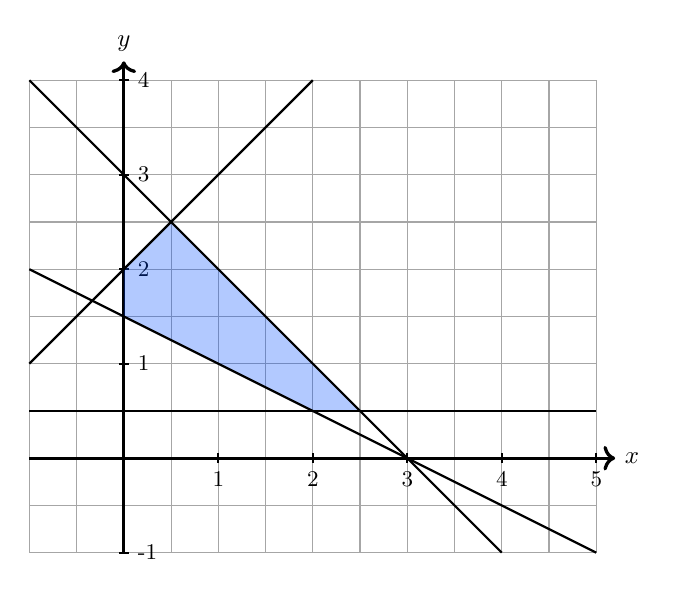
\begin{tikzpicture}[thick,scale=1.2, every node/.style={scale=0.9}]
	
	\draw[gray!70, thin, step=0.5] (-1,-1) grid (5,4);
	\draw[very thick,->] (-1,0) -- (5.2,0) node[right] {$x$};
	\draw[very thick,->] (0,-1) -- (0,4.2) node[above] {$y$};
	
	\foreach \x in {1,...,5} \draw (\x,0.05) -- (\x,-0.05) node[below] {\small\x};
	\foreach \y in {1,...,4} \draw (-0.05,\y) -- (0.05,\y) node[right] {\small\y};
	\foreach \y in {-1,...,-1} \draw (-0.05,\y) -- (0.05,\y) node[right] {\small\y};
	
	\fill[blue!70!cyan,opacity=0.3] (0,2) -- (0.5,2.5) -- (2.5,0.5) -- (2,0.5) -- (0,1.5) -- cycle;
	
	\draw (-1,4) -- node[below,sloped] {} (4,-1);
%	\draw (1,-3) -- (3,1) -- node[below left,sloped] {} (4.5,4);
%	\draw (-1,1) -- node[above,sloped] {} (5,4);
	\draw (-1,2) -- node[above,sloped] {} (5,-1);
	\draw (-1,1) -- node[above,sloped] {} (2,4);
	\draw (-1,0.5) -- node[above,sloped] {} (5,0.5);
	
	\end{tikzpicture} 
\end{minipage}
\begin{minipage}[b]{0.50\textwidth}

Find the maximum value of the objective function 	$M=10-3x+2y$ in this feasible region. Show your work step-by-step.
\fillwithdottedlines{5cm}
\end{minipage}

\fillwithdottedlines{2cm}

	\question[2] At a certain vineyard it is found that each grape vine produces about 10 pounds of grapes in a season when about 600 vines are planted per acre. For each additional vine that is planted, the production of each vine decreases by about 1 percent. So the number of pounds of grapes produced per acre is modeled by
	$\displaystyle A(n) = (600 + n)(10 - 0.01n)$
	where $n$ is the number of additional vines planted. Find the number of vines that should be planted to maximize grape production. Show your work step-by-step.
	\fillwithdottedlines{5cm}
\question A tank holds 100 gallons of water, which drains from a leak at the bottom, causing the tank to drain in 40 minutes. The volume of water remaining in the tank after $t$ minutes is $\displaystyle V(t)=100\left (1-\frac{t}{40}\right )^2$.
\begin{parts}
	\part[2]  Find $\displaystyle V^{-1}(100)$. Show your work step by step.
	\fillwithdottedlines{2cm} 
	\part[1] Does $\displaystyle V^{-1}(100)$ represent time or volume? \dotfill
\end{parts} 	
	%\newpage	
\question The function $r(x)$ is obtained by applying the following transformations on $\displaystyle f(x)=x^2$: 

 First, $f(x)$ is reflected around the $x$ axis;
	 Then, the resulting function is shifted horizontally 9 units to the left, and
 Finally, the resulting function is moved vertically 81 units upward.

\begin{parts}
\part[2] Write the formula for $r(x)$.	\dotfill
\fillwithdottedlines{1cm}

\part[1] Write the range of $r(x)$ in interval form. \dotfill
	
	\end{parts}


\question[4]  Draw a rational function that has all of the following properties.
\begin{itemize}
	\item $x=-4$ and $x=4$ are the two vertical asymptotes;
	\item The tails of the graph of $f(x)$ near $x=-4$ go in opposite directions;
	\item The tails of the graph of $f(x)$ near $x=4$ go in the same direction;
	\item $(3,0)$ is the only $x$-intercept, and the graph goes across the $x$-axis at this $x$-intercept;
	\item The $y$-intercept is $(0,-1)$;
	\item The horizontal asymptote is $\displaystyle y=\frac{1}{2}$.
\end{itemize}
Label all asymptotes and intercepts.



\begin{tikzpicture}
\draw[gray!50, thin, step=0.5] (-7,-3) grid (7,3);
\end{tikzpicture}




	\question Consider the following functions:
	$\displaystyle f(x) = x-2$,     $\displaystyle g(x) = \sqrt{x}$ 
	\begin{parts}
		\part[1] Find $\displaystyle f(4)+g(4)$. \dotfill
		\part[1] Find $\displaystyle \frac{g(4)}{f(4)}$ \dotfill
		\part[1] Write the domain of $\displaystyle f(x)+g(x)$ in interval form. \dotfill
		\part[1] Write the domain of $\displaystyle \frac{g(x)}{f(x)}$ in interval form. \dotfill
		\part[1] Write the domain of $\displaystyle \frac{f(x)}{g(x)}$ in interval form. \dotfill
		\part[2] Why isn't $\displaystyle \frac{g(x)}{f(x)}$ a rational function?
		\fillwithdottedlines{2cm}
		
	\end{parts}

\end{questions}
\newpage
\thispagestyle{empty}


\setlength\fboxrule{2pt}\setlength\fboxsep{2mm}
\fbox{This page is intentionally left blank.} You may use it as scrap paper for your calculations.
\end{document}                 